\FloatBarrier

% Problema \getNumeroProblema (Basato su Kharef P35)
\begin{table}[htbp]
  \centering
  \renewcommand{\arraystretch}{1.5}
  \begin{tabular}{|>{\raggedright\arraybackslash}p{7.5cm}|>{\raggedright\arraybackslash}p{7.5cm}|}
    \hline
    \rowcolor{green!30}
    \multicolumn{2}{|c|}{\textbf{Problema \getNumeroProblema}} \\
    \hline
    \textbf{Descrizione} & Il sistema manca di strumenti organizzativi per la gestione di grandi quantità di documenti. Non esistono cartelle, sottocartelle personalizzate nella pagina "Esplora Appunti", rendendo l'uso ingestibile nel lungo periodo. \\
    \hline
    \textbf{Pagina del sito} & Esplora Appunti \\
    \hline
    \textbf{Principi violati} & 6 (Assicurare flessibilità ed efficienza d’uso); 7 (Visualizzare tutte e sole le informazioni necessarie) \\
    \hline
    \textbf{Grado di severità} & 3 (Problema rilevante) \\
    \hline
    \textbf{Nome del valutatore} & Kharef \\
    \hline
  \end{tabular}
\end{table}

% Problema \getNumeroProblema (Basato su Kharef P36)
\begin{table}[htbp]
  \centering
  \renewcommand{\arraystretch}{1.5}
  \begin{tabular}{|>{\raggedright\arraybackslash}p{7.5cm}|>{\raggedright\arraybackslash}p{7.5cm}|}
    \hline
    \rowcolor{green!30}
    \multicolumn{2}{|c|}{\textbf{Problema \getNumeroProblema}} \\
    \hline
    \textbf{Descrizione} & L'utente non può selezionare più documenti o trascrizioni o audio contemporaneamente per eseguire azioni comuni (es. caricare, eliminare, rendere pubblici/privati). \\
    \hline
    \textbf{Pagina del sito} & I Miei Appunti \\
    \hline
    \textbf{Principi violati} & 6 (Assicurare flessibilità ed efficienza d’uso) \\
    \hline
    \textbf{Grado di severità} & 2 (Problema secondario) \\
    \hline
    \textbf{Nome del valutatore} & Kharef \\
    \hline
  \end{tabular}
\end{table}

% Problema \getNumeroProblema (Basato su Kharef P38)
\begin{table}[htbp]
  \centering
  \renewcommand{\arraystretch}{1.5}
  \begin{tabular}{|>{\raggedright\arraybackslash}p{7.5cm}|>{\raggedright\arraybackslash}p{7.5cm}|}
    \hline
    \rowcolor{green!30}
    \multicolumn{2}{|c|}{\textbf{Problema \getNumeroProblema}} \\
    \hline
    \textbf{Descrizione} & Le trascrizioni generate dallo "Sbobinatore AI" mancano di struttura semantica. Sono presentate come un unico blocco di testo, senza timestamp che colleghino le frasi al punto corrispondente nel file audio. \\
    \hline
    \textbf{Pagina del sito} & Sbobinatore AI \\
    \hline
    \textbf{Principi violati} & 2 (Adeguare il sistema al mondo reale); 5 (Riconoscimento piuttosto che uso della memoria dell’utente) \\
    \hline
    \textbf{Grado di severità} & 3 (Problema rilevante) \\
    \hline
    \textbf{Screen} & 
    \vspace{10pt}
    \hspace*{\fill}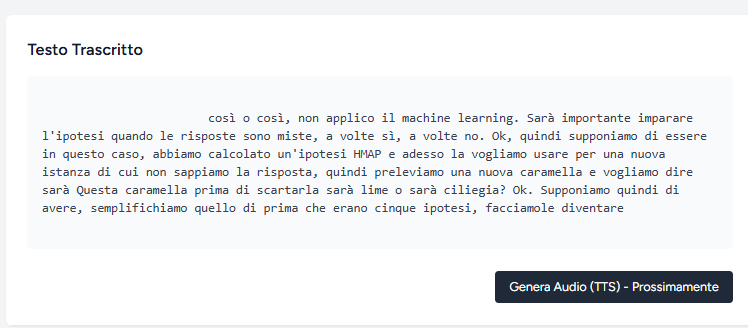
\includegraphics[width=6.5cm]{Screenshots/foglio3/problema85.png}\hspace*{\fill}
    \vspace{10pt}
    \\
    \hline
    \textbf{Nome del valutatore} & Kharef \\
    \hline
  \end{tabular}
\end{table}

% Problema \getNumeroProblema (Basato su Kharef P39)
\begin{table}[htbp]
  \centering
  \renewcommand{\arraystretch}{1.5}
  \begin{tabular}{|>{\raggedright\arraybackslash}p{7.5cm}|>{\raggedright\arraybackslash}p{7.5cm}|}
    \hline
    \rowcolor{green!30}
    \multicolumn{2}{|c|}{\textbf{Problema \getNumeroProblema}} \\
    \hline
    \textbf{Descrizione} & La ricerca è superficiale e non indicizza il contenuto dei file. Viene effettuata solo sui metadati (titolo, materia, descrizione), ignorando il testo contenuto all'interno dei file caricati. \\
    \hline
    \textbf{Pagina del sito} & Esplora Appunti \\
    \hline
    \textbf{Principi violati} & 2 (Adeguare il sistema al mondo reale); 7 (Visualizzare tutte e sole le informazioni necessarie) \\
    \hline
    \textbf{Grado di severità} & 2 (Problema secondario) \\
    \hline
    \textbf{Nome del valutatore} & Kharef \\
    \hline
  \end{tabular}
\end{table}

% Problema \getNumeroProblema (Basato su Kharef P40)
\begin{table}[htbp]
  \centering
  \renewcommand{\arraystretch}{1.5}
  \begin{tabular}{|>{\raggedright\arraybackslash}p{7.5cm}|>{\raggedright\arraybackslash}p{7.5cm}|}
    \hline
    \rowcolor{green!30}
    \multicolumn{2}{|c|}{\textbf{Problema \getNumeroProblema}} \\
    \hline
    \textbf{Descrizione} & La piattaforma non offre alcun tipo di funzionalità offline. L'accesso ai propri appunti, anche per la sola lettura, è completamente impedito senza una connessione internet stabile. \\
    \hline
    \textbf{Pagina del sito} & Globale \\
    \hline
    \textbf{Principi violati} & 3 (Controllo dell’utente e libertà) \\
    \hline
    \textbf{Grado di severità} & 2 (Problema secondario) \\
    \hline
    \textbf{Nome del valutatore} & Kharef \\
    \hline
  \end{tabular}
\end{table}

% Problema \getNumeroProblema (Basato su Kharef P41)
\begin{table}[htbp]
  \centering
  \renewcommand{\arraystretch}{1.5}
  \begin{tabular}{|>{\raggedright\arraybackslash}p{7.5cm}|>{\raggedright\arraybackslash}p{7.5cm}|}
    \hline
    \rowcolor{green!30}
    \multicolumn{2}{|c|}{\textbf{Problema \getNumeroProblema}} \\
    \hline
    \textbf{Descrizione} & Non c'è un modo per l'utente di vedere quali altri documenti ha caricato l'autore di un appunto, né ci sono suggerimenti automatici del tipo "Chi ha consultato questo appunto ha consultato anche...". \\
    \hline
    \textbf{Pagina del sito} & Esplora Appunti \\
    \hline
    \textbf{Principi violati} & 7 (Visualizzare tutte e sole le informazioni necessarie) \\
    \hline
    \textbf{Grado di severità} & 2 (Problema secondario) \\
    \hline
    \textbf{Nome del valutatore} & Kharef \\
    \hline
  \end{tabular}
\end{table}

% Problema \getNumeroProblema (Basato su Kharef P42)
\begin{table}[htbp]
  \centering
  \renewcommand{\arraystretch}{1.5}
  \begin{tabular}{|>{\raggedright\arraybackslash}p{7.5cm}|>{\raggedright\arraybackslash}p{7.5cm}|}
    \hline
    \rowcolor{green!30}
    \multicolumn{2}{|c|}{\textbf{Problema \getNumeroProblema}} \\
    \hline
    \textbf{Descrizione} & Il sistema non gestisce i contenuti duplicati. Se dieci studenti caricano lo stesso PDF, la pagina "Esplora Appunti" mostrerà dieci risultati identici, inquinando i risultati di ricerca. \\
    \hline
    \textbf{Pagina del sito} & Esplora Appunti \\
    \hline
    \textbf{Principi violati} & 1 (Far vedere lo stato del sistema); 8 (Prevenire gli errori) \\
    \hline
    \textbf{Grado di severità} & 4 (Catastrofe di usabilità) \\
    \hline
    \textbf{Screen} & 
    \vspace{10pt}
    \hspace*{\fill}
\includegraphics[width=6.5cm]{Screenshots/foglio3/problema93.png}\hspace*{\fill}
    \vspace{10pt}
    \\
    \hline
    \textbf{Nome del valutatore} & Kharef \\
    \hline
  \end{tabular}
\end{table}

% Problema \getNumeroProblema (Basato su Kharef P47)
\begin{table}[htbp]
  \centering
  \renewcommand{\arraystretch}{1.5}
  \begin{tabular}{|>{\raggedright\arraybackslash}p{7.5cm}|>{\raggedright\arraybackslash}p{7.5cm}|}
    \hline
    \rowcolor{green!30}
    \multicolumn{2}{|c|}{\textbf{Problema \getNumeroProblema}} \\
    \hline
    \textbf{Descrizione} & La lista dei commenti in una pagina di dettaglio non è paginata. Se un documento popolare riceve molti commenti, la pagina diventa estremamente lunga e lenta da caricare. \\
    \hline
    \textbf{Pagina del sito} & I Miei Appunti - Visualizzazione Documento \\
    \hline
    \textbf{Principi violati} & 6 (Assicurare flessibilità ed efficienza d’uso); 7 (Visualizzare tutte e sole le informazioni necessarie) \\
    \hline
    \textbf{Grado di severità} & 3 (Problema rilevante) \\
    \hline
    \textbf{Screen} &
    \vspace{10pt}
    \hspace*{\fill}
\includegraphics[height=6cm, keepaspectratio]{Screenshots/foglio3/problema97.png}\hspace*{\fill}
    \vspace{10pt}
    \\
    \hline
    \textbf{Nome del valutatore} & Kharef \\
    \hline
  \end{tabular}
\end{table}

% Problema \getNumeroProblema (Basato su Kharef P48 - Violazione Sicurezza)
\begin{table}[htbp]
  \centering
  \renewcommand{\arraystretch}{1.5}
  \begin{tabular}{|>{\raggedright\arraybackslash}p{7.5cm}|>{\raggedright\arraybackslash}p{7.5cm}|}
    \hline
    \rowcolor{green!30}
    \multicolumn{2}{|c|}{\textbf{Problema \getNumeroProblema}} \\
    \hline
    \textbf{Descrizione} & Non esiste alcun meccanismo di autorizzazione per l'accesso ai file caricati. Se un utente indovina l'URL diretto a un file, può scaricarlo liberamente, anche se il documento è contrassegnato come "privato" nell'interfaccia. \\
    \hline
    \textbf{Pagina del sito} & Globale \\
    \hline
    \textbf{Principi violati} & 8 (Prevenire gli errori) \\
    \hline
    \textbf{Grado di severità} & 4 (Catastrofe di usabilità) \\
    \hline
    \textbf{Nome del valutatore} & Kharef \\
    \hline
  \end{tabular}
\end{table}

% Problema \getNumeroProblema
\begin{table}[htbp]
  \centering
  \renewcommand{\arraystretch}{1.5}
  \begin{tabular}{|>{\raggedright\arraybackslash}p{7.5cm}|>{\raggedright\arraybackslash}p{7.5cm}|}
    \hline
    \rowcolor{green!30}
    \multicolumn{2}{|c|}{\textbf{Problema \getNumeroProblema}} \\
    \hline
    \textbf{Descrizione} & Nella homepage il pulsante "Accedi" è meno evidente rispetto al pulsante "Inizia Subito", e può far pensare che non sia un pulsante. \\
    \hline
    \textbf{Pagina del sito} & Homepage \\
    \hline
    \textbf{Principi violati} & 4 (Assicurare consistenza); 5 (Riconoscimento piuttosto che uso della memoria dell'utente) \\
    \hline
    \textbf{Grado di severità} & 1 (Problema accessorio) \\
    \hline
    \textbf{Screen} &
    \vspace{10pt}
    \hspace*{\fill}
\includegraphics[width=6.5cm]{Screenshots/foglio4/Problema104.png}\hspace*{\fill}
    \vspace{10pt}
    \\
    \hline
    \textbf{Nome del valutatore} & Rinaldi \\
    \hline
  \end{tabular}
\end{table}

% Problema \getNumeroProblema
\begin{table}[htbp]
  \centering
  \renewcommand{\arraystretch}{1.5}
  \begin{tabular}{|>{\raggedright\arraybackslash}p{7.5cm}|>{\raggedright\arraybackslash}p{7.5cm}|}
    \hline
    \rowcolor{green!30}
    \multicolumn{2}{|c|}{\textbf{Problema \getNumeroProblema}} \\
    \hline
    \textbf{Descrizione} & Nel form di login la funzione "Ricordami" non è operativa. \\
    \hline
    \textbf{Pagina del sito} & Login \\
    \hline
    \textbf{Principi violati} & 1 (Far vedere lo stato del sistema); 8 (Prevenire gli errori) \\
    \hline
    \textbf{Grado di severità} & 4 (Catastrofe di usabilità) \\
    \hline
    \textbf{Nome del valutatore} & Rinaldi \\
    \hline
  \end{tabular}
\end{table}

% Problema \getNumeroProblema
\begin{table}[htbp]
  \centering
  \renewcommand{\arraystretch}{1.5}
  \begin{tabular}{|>{\raggedright\arraybackslash}p{7.5cm}|>{\raggedright\arraybackslash}p{7.5cm}|}
    \hline
    \rowcolor{green!30}
    \multicolumn{2}{|c|}{\textbf{Problema \getNumeroProblema}} \\
    \hline
    \textbf{Descrizione} & La funzione di cambio password consente di inserire password con meno di otto caratteri senza mostrare alcun messaggio di errore. Tuttavia, la nuova password non viene effettivamente salvata, garantendo i nuovi accessi ancora con la password vecchia. \\
    \hline
    \textbf{Pagina del sito} & Profilo - Aggiornamento Password \\
    \hline
    \textbf{Principi violati} & 1 (Far vedere lo stato del sistema); 8 (Prevenire gli errori) \\
    \hline
    \textbf{Grado di severità} & 4 (Catastrofe di usabilità) \\
    \hline
    \textbf{Nome del valutatore} & Rinaldi \\
    \hline
  \end{tabular}
\end{table}

% Problema \getNumeroProblema
\begin{table}[htbp]
  \centering
  \renewcommand{\arraystretch}{1.5}
  \begin{tabular}{|>{\raggedright\arraybackslash}p{7.5cm}|>{\raggedright\arraybackslash}p{7.5cm}|}
    \hline
    \rowcolor{green!30}
    \multicolumn{2}{|c|}{\textbf{Problema \getNumeroProblema}} \\
    \hline
    \textbf{Descrizione} & Nella sezione "Esami in programma" è possibile inserire un esame con una data antecedente a quella corrente; tale esame non viene poi visualizzato nella pagina principale. \\
    \hline
    \textbf{Pagina del sito} & StudyFlow AI\\
    \hline
    \textbf{Principi violati} & 2 (Adeguare il sistema al mondo reale); 7 (Visualizzare tutte e sole le informazioni necessarie); 9 (Permettere all'utente di correggere gli errori e non solo di rilevarli) \\
    \hline
    \textbf{Grado di severità} & 3 (Problema rilevante) \\
    \hline
    \textbf{Screen} &
    \vspace{10pt}
    \hspace*{\fill}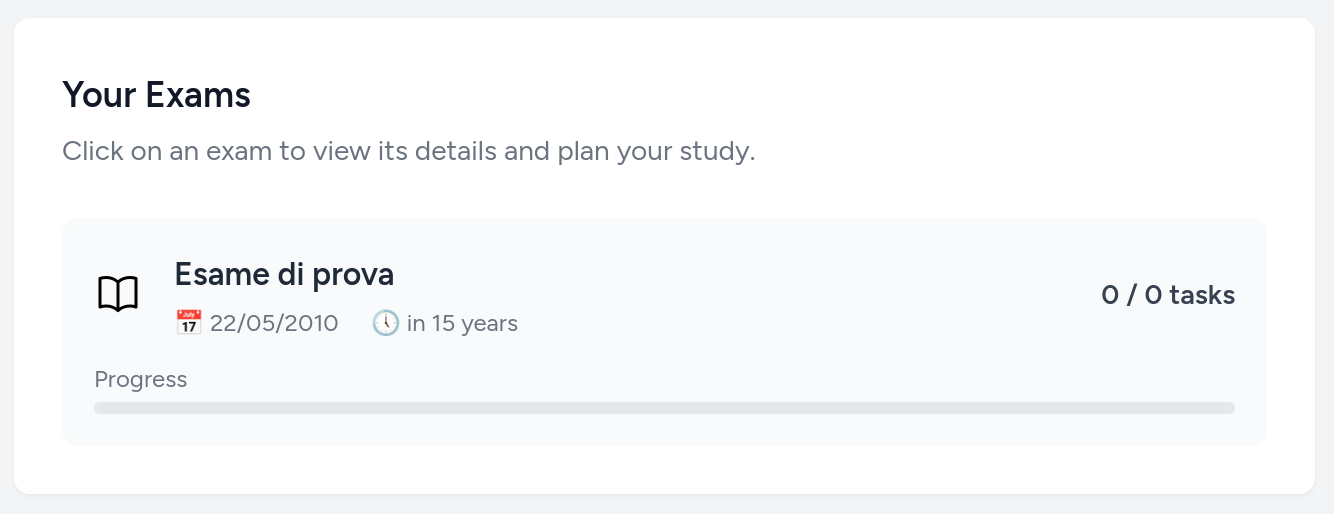
\includegraphics[width=6.5cm]{Screenshots/foglio4/Problema107.png}\hspace*{\fill}
    \vspace{10pt}
    \\
    \hline
    \textbf{Nome del valutatore} & Rinaldi \\
    \hline
  \end{tabular}
\end{table}

% Problema \getNumeroProblema
\begin{table}[htbp]
  \centering
  \renewcommand{\arraystretch}{1.5}
  \begin{tabular}{|>{\raggedright\arraybackslash}p{7.5cm}|>{\raggedright\arraybackslash}p{7.5cm}|}
    \hline
    \rowcolor{green!30}
    \multicolumn{2}{|c|}{\textbf{Problema \getNumeroProblema}} \\
    \hline
    \textbf{Descrizione} & Nella visualizzazione dei dettagli di un esame, cliccando il pulsante "Aggiungi materiale esistente", viene mostrato il messaggio "Tutti i tuoi documenti sono già stati collegati!" anche quando non sono presenti materiali nel proprio repository. \\
    \hline
    \textbf{Pagina del sito} & StudyFlow AI \\
    \hline
    \textbf{Principi violati} & 1 (Far vedere lo stato del sistema); 9 (Permettere all’utente di correggere gli errori e non solo di rilevarli) \\
    \hline
    \textbf{Grado di severità} & 2 (Problema secondario) \\
    \hline
    \textbf{Screen} &
    \vspace{10pt}
    \hspace*{\fill}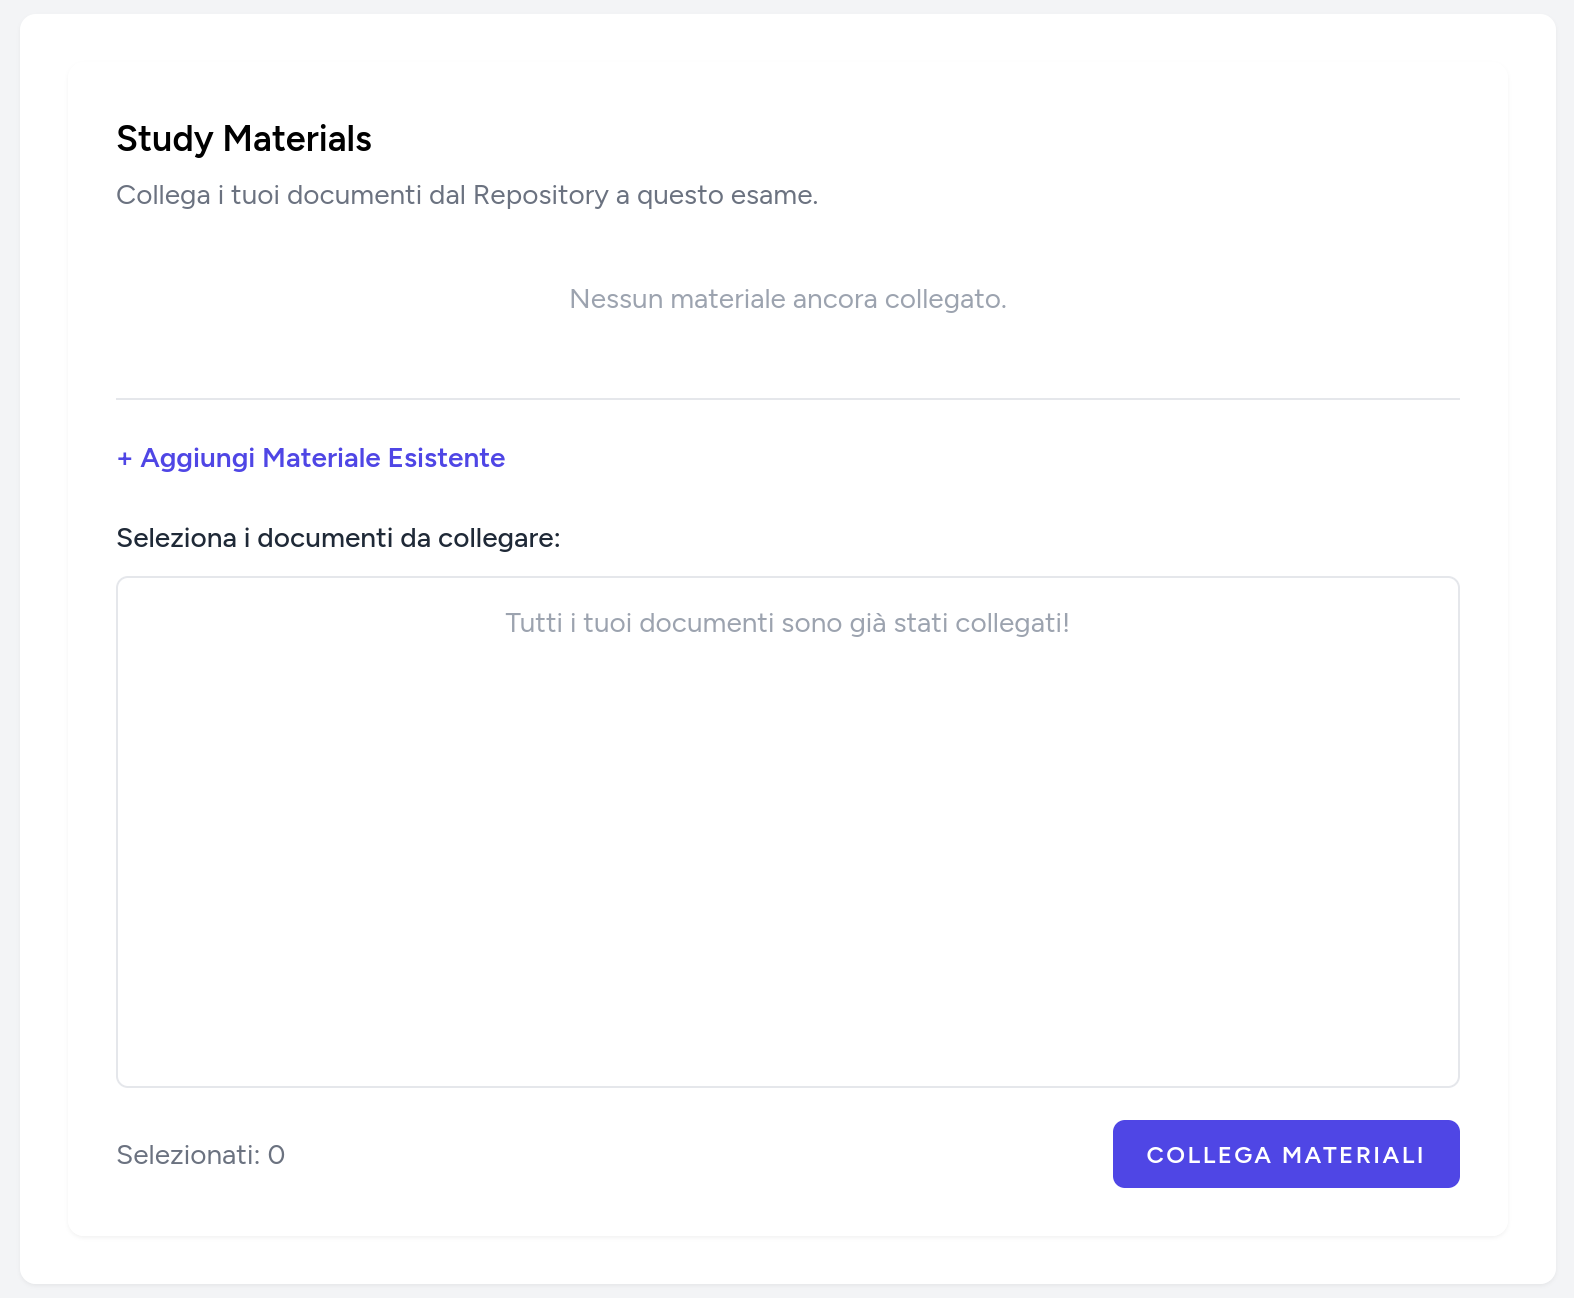
\includegraphics[width=6.5cm]{Screenshots/foglio4/Problema108.png}\hspace*{\fill}
    \vspace{10pt}
    \\
    \hline
    \textbf{Nome del valutatore} & Rinaldi \\
    \hline
  \end{tabular}
\end{table}

% Problema \getNumeroProblema
\begin{table}[htbp]
  \centering
  \renewcommand{\arraystretch}{1.5}
  \begin{tabular}{|>{\raggedright\arraybackslash}p{7.5cm}|>{\raggedright\arraybackslash}p{7.5cm}|}
    \hline
    \rowcolor{green!30}
    \multicolumn{2}{|c|}{\textbf{Problema \getNumeroProblema}} \\
    \hline
    \textbf{Descrizione} &  Nella visualizzazione dei dettagli di un esame, cliccando il pulsante "Aggiungi materiale esistente", quando non sono presenti materiali nel proprio repository, il pulsante "Collega materiali" compare senza alcuna funzione attiva. \\
    \hline
    \textbf{Pagina del sito} & StudyFlow AI \\
    \hline
    \textbf{Principi violati} & 7 (Visualizzare tutte e sole le informazioni necessarie) \\
    \hline
    \textbf{Grado di severità} & 1 (Problema accessorio) \\
    \hline
    \textbf{Screen} &
    \vspace{10pt}
    \hspace*{\fill}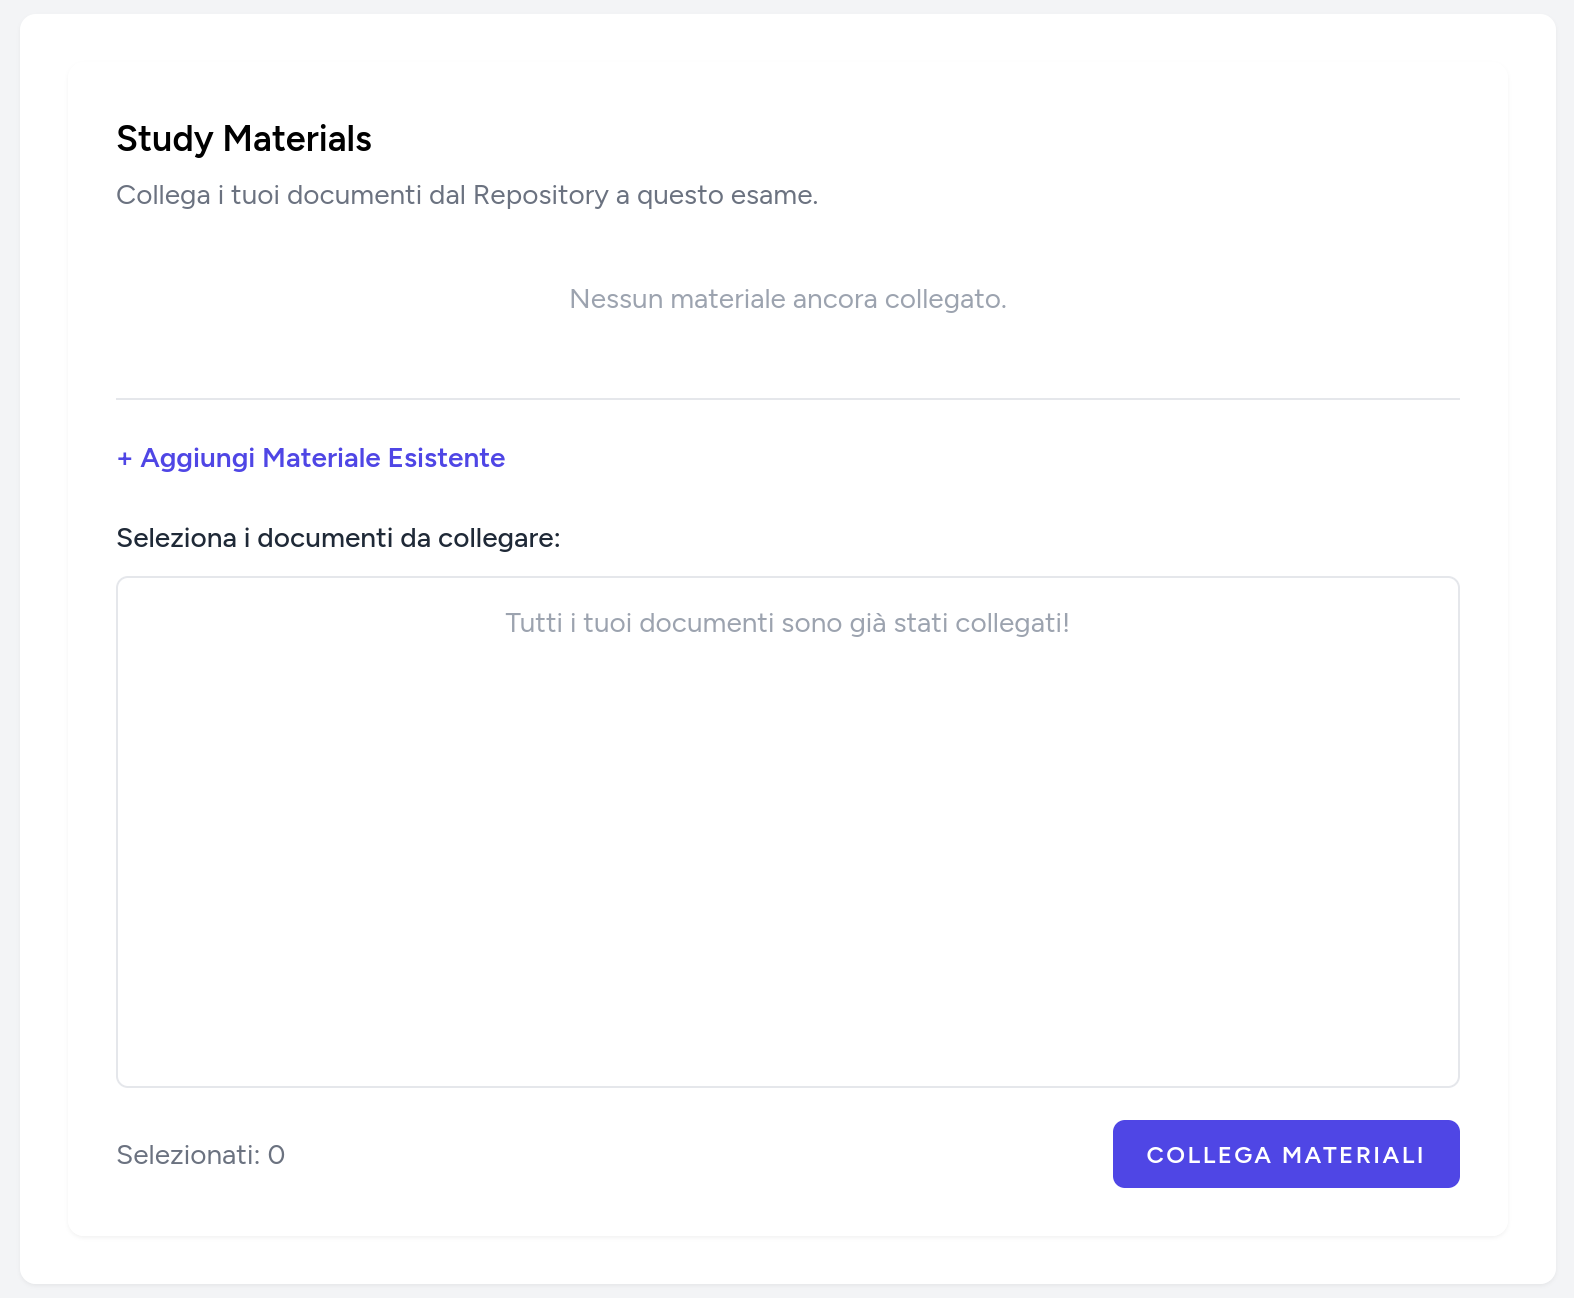
\includegraphics[width=6.5cm]{Screenshots/foglio4/Problema109.png}\hspace*{\fill}
    \vspace{10pt}
    \\
    \hline
    \textbf{Nome del valutatore} & Rinaldi \\
    \hline
  \end{tabular}
\end{table}

% Problema \getNumeroProblema
\begin{table}[htbp]
  \centering
  \renewcommand{\arraystretch}{1.5}
  \begin{tabular}{|>{\raggedright\arraybackslash}p{7.5cm}|>{\raggedright\arraybackslash}p{7.5cm}|}
    \hline
    \rowcolor{green!30}
    \multicolumn{2}{|c|}{\textbf{Problema \getNumeroProblema}} \\
    \hline
    \textbf{Descrizione} &  Nei dettagli di un esame se si elimina una task compare un avviso che può risultare "strano" all'utente in cui viene chiesto se si è sicuri di voler eliminare l'attività.\\
    \hline
    \textbf{Pagina del sito} & StudyFlow AI \\
    \hline
    \textbf{Principi violati} & 4 (Assicurare consistenza); 6 (Assicurare flessibilità ed efficienza d’uso ) \\
    \hline
    \textbf{Grado di severità} & 3 (Problema rilevante) \\
    \hline
    \textbf{Screen} &
    \vspace{10pt}
    \hspace*{\fill}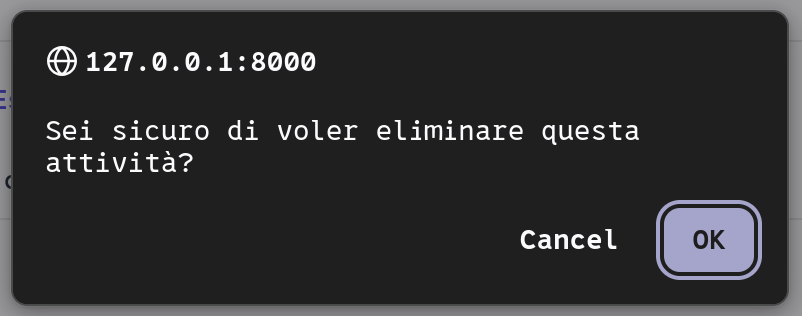
\includegraphics[width=6.5cm]{Screenshots/foglio4/Problema110.png}\hspace*{\fill}
    \vspace{10pt}
    \\
    \hline
    \textbf{Nome del valutatore} & Rinaldi \\
    \hline
  \end{tabular}
\end{table}

% Problema \getNumeroProblema
\begin{table}[htbp]
  \centering
  \renewcommand{\arraystretch}{1.5}
  \begin{tabular}{|>{\raggedright\arraybackslash}p{7.5cm}|>{\raggedright\arraybackslash}p{7.5cm}|}
    \hline
    \rowcolor{green!30}
    \multicolumn{2}{|c|}{\textbf{Problema \getNumeroProblema}} \\
    \hline
    \textbf{Descrizione} &  Nella sezione "Exam Details" è presente una sezione del calendario non funzionante. \\
    \hline
    \textbf{Pagina del sito} & StudyFlow AI \\
    \hline
    \textbf{Principi violati} & 4 (Assicurare consistenza) \\
    \hline
    \textbf{Grado di severità} & 4 (Catastrofe di usabilità) \\
    \hline
    \textbf{Screen} &
    \vspace{10pt}
    \hspace*{\fill}
\includegraphics[width=6.5cm]{Screenshots/foglio4/Problema111.png}\hspace*{\fill}
    \vspace{10pt}
    \\
    \hline
    \textbf{Nome del valutatore} & Rinaldi, Kharef \\
    \hline
  \end{tabular}
\end{table}


% Problema \getNumeroProblema
\begin{table}[htbp]
  \centering
  \renewcommand{\arraystretch}{1.5}
  \begin{tabular}{|>{\raggedright\arraybackslash}p{7.5cm}|>{\raggedright\arraybackslash}p{7.5cm}|}
    \hline
    \rowcolor{green!30}
    \multicolumn{2}{|c|}{\textbf{Problema \getNumeroProblema}} \\
    \hline
    \textbf{Descrizione} &   Durante il caricamento di un file è obbligatorio inserire tutti i dettagli del documento, anche se non si intende renderlo pubblico. \\
    \hline
    \textbf{Pagina del sito} & I Miei Appunti - Caricamento file \\
    \hline
    \textbf{Principi violati} & 6 (Assicurare flessibilità ed efficienza d'uso); 7 (Visualizzare tutte e sole le informazioni necessarie) \\
    \hline
    \textbf{Grado di severità} & 1 (Problema accessorio) \\
    \hline
    \textbf{Nome del valutatore} & Rinaldi \\
    \hline
  \end{tabular}
\end{table}

% Problema \getNumeroProblema
\begin{table}[htbp]
  \centering
  \renewcommand{\arraystretch}{1.5}
  \begin{tabular}{|>{\raggedright\arraybackslash}p{7.5cm}|>{\raggedright\arraybackslash}p{7.5cm}|}
    \hline
    \rowcolor{green!30}
    \multicolumn{2}{|c|}{\textbf{Problema \getNumeroProblema}} \\
    \hline
    \textbf{Descrizione} & La sezione "Your Exams" è accessibile tramite il pulsante "StudyFlow AI", collocato nella sezione "Strumenti AI", il che risulta poco pertinente rispetto alla sua funzione. \\
    \hline
    \textbf{Pagina del sito} & StudyFlow AI\\
    \hline
    \textbf{Principi violati} & 4 (Assicurare consistenza) \\
    \hline
    \textbf{Grado di severità} & 1 (Problema accessorio) \\
    \hline
    \textbf{Screen} &
    \vspace{10pt}
    \hspace*{\fill}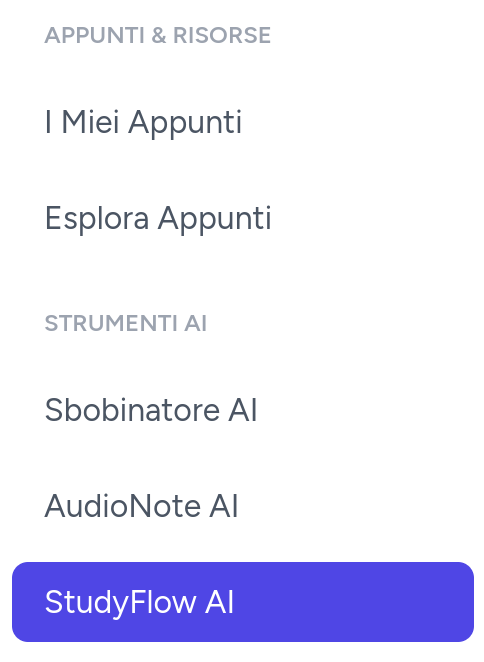
\includegraphics[width=6.5cm]{Screenshots/foglio4/Problema113.png}\hspace*{\fill}
    \vspace{10pt}
    \\
    \hline
    \textbf{Nome del valutatore} & Rinaldi \\
    \hline
  \end{tabular}
\end{table}

% Problema \getNumeroProblema
\begin{table}[htbp]
  \centering
  \renewcommand{\arraystretch}{1.5}
  \begin{tabular}{|>{\raggedright\arraybackslash}p{7.5cm}|>{\raggedright\arraybackslash}p{7.5cm}|}
    \hline
    \rowcolor{green!30}
    \multicolumn{2}{|c|}{\textbf{Problema \getNumeroProblema}} \\
    \hline
    \textbf{Descrizione} & In "Your Exams" non c'è la possibilità di eliminare un esame, ma solo di crearne di nuovi e aggiungerli alla lista. \\
    \hline
    \textbf{Pagina del sito} & StudyFlow AI \\
    \hline
    \textbf{Principi violati} & 2 (Adeguare il sistema al mondo reale); 3 (Controllo dell’utente e libertà); 9 (Permettere all’utente di correggere gli errori e non solo di rilevarli) \\
    \hline
    \textbf{Grado di severità} & 3 (Problema rilevante) \\
    \hline
    \textbf{Nome del valutatore} & Rinaldi \\
    \hline
  \end{tabular}
\end{table}

% Problema \getNumeroProblema
\begin{table}[htbp]
  \centering
  \renewcommand{\arraystretch}{1.5}
  \begin{tabular}{|>{\raggedright\arraybackslash}p{7.5cm}|>{\raggedright\arraybackslash}p{7.5cm}|}
    \hline
    \rowcolor{green!30}
    \multicolumn{2}{|c|}{\textbf{Problema \getNumeroProblema}} \\
    \hline
    \textbf{Descrizione} & Durante l'upload di un file vengono richiesti dettagli come università e dipartimento tramite menu a tendina che consentono di selezionare la voce "Seleziona . . ." che non dovrebbe essere selezionabile. \\
    \hline
    \textbf{Pagina del sito} & I Miei Appunti - Caricamento File \\
    \hline
    \textbf{Principi violati} & 7 (Visualizzare tutte e sole le informazioni necessarie); 8 (Prevenire gli errori) \\
    \hline
    \textbf{Grado di severità} & 2 (Problema secondario) \\
    \hline
    \textbf{Screen} &
    \vspace{10pt}
    \hspace*{\fill}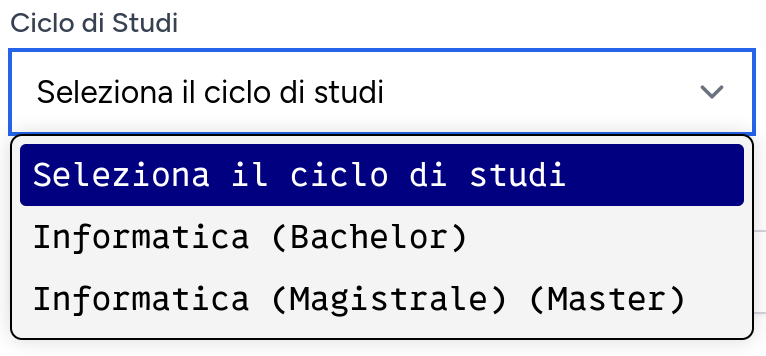
\includegraphics[width=6.5cm]{Screenshots/foglio4/Problema115.png}\hspace*{\fill}
    \vspace{10pt}
    \\
    \hline
    \textbf{Nome del valutatore} & Rinaldi \\
    \hline
  \end{tabular}
\end{table}

% Problema \getNumeroProblema
\begin{table}[htbp]
  \centering
  \renewcommand{\arraystretch}{1.5}
  \begin{tabular}{|>{\raggedright\arraybackslash}p{7.5cm}|>{\raggedright\arraybackslash}p{7.5cm}|}
    \hline
    \rowcolor{green!30}
    \multicolumn{2}{|c|}{\textbf{Problema \getNumeroProblema}} \\
    \hline
    \textbf{Descrizione} & Durante l'upload di un file vengono richiesti dettagli come università e dipartimento tramite menu a tendina e, in alcuni casi, la mancata selezione non genera alcun messaggio/avviso di errore al momento del click del pulsante di salvataggio. \\
    \hline
    \textbf{Pagina del sito} & I Miei Appunti - Caricamento File \\
    \hline
    \textbf{Principi violati} & 1 (Far vedere lo stato del sistema); 8 (Prevenire gli errori); 9 (Permettere all'utente di correggere gli errori e non solo di rilevarli) \\
    \hline
    \textbf{Grado di severità} & 3 (Problema rilevante) \\
    \hline
    \textbf{Screen} &
    \vspace{10pt}
    \hspace*{\fill}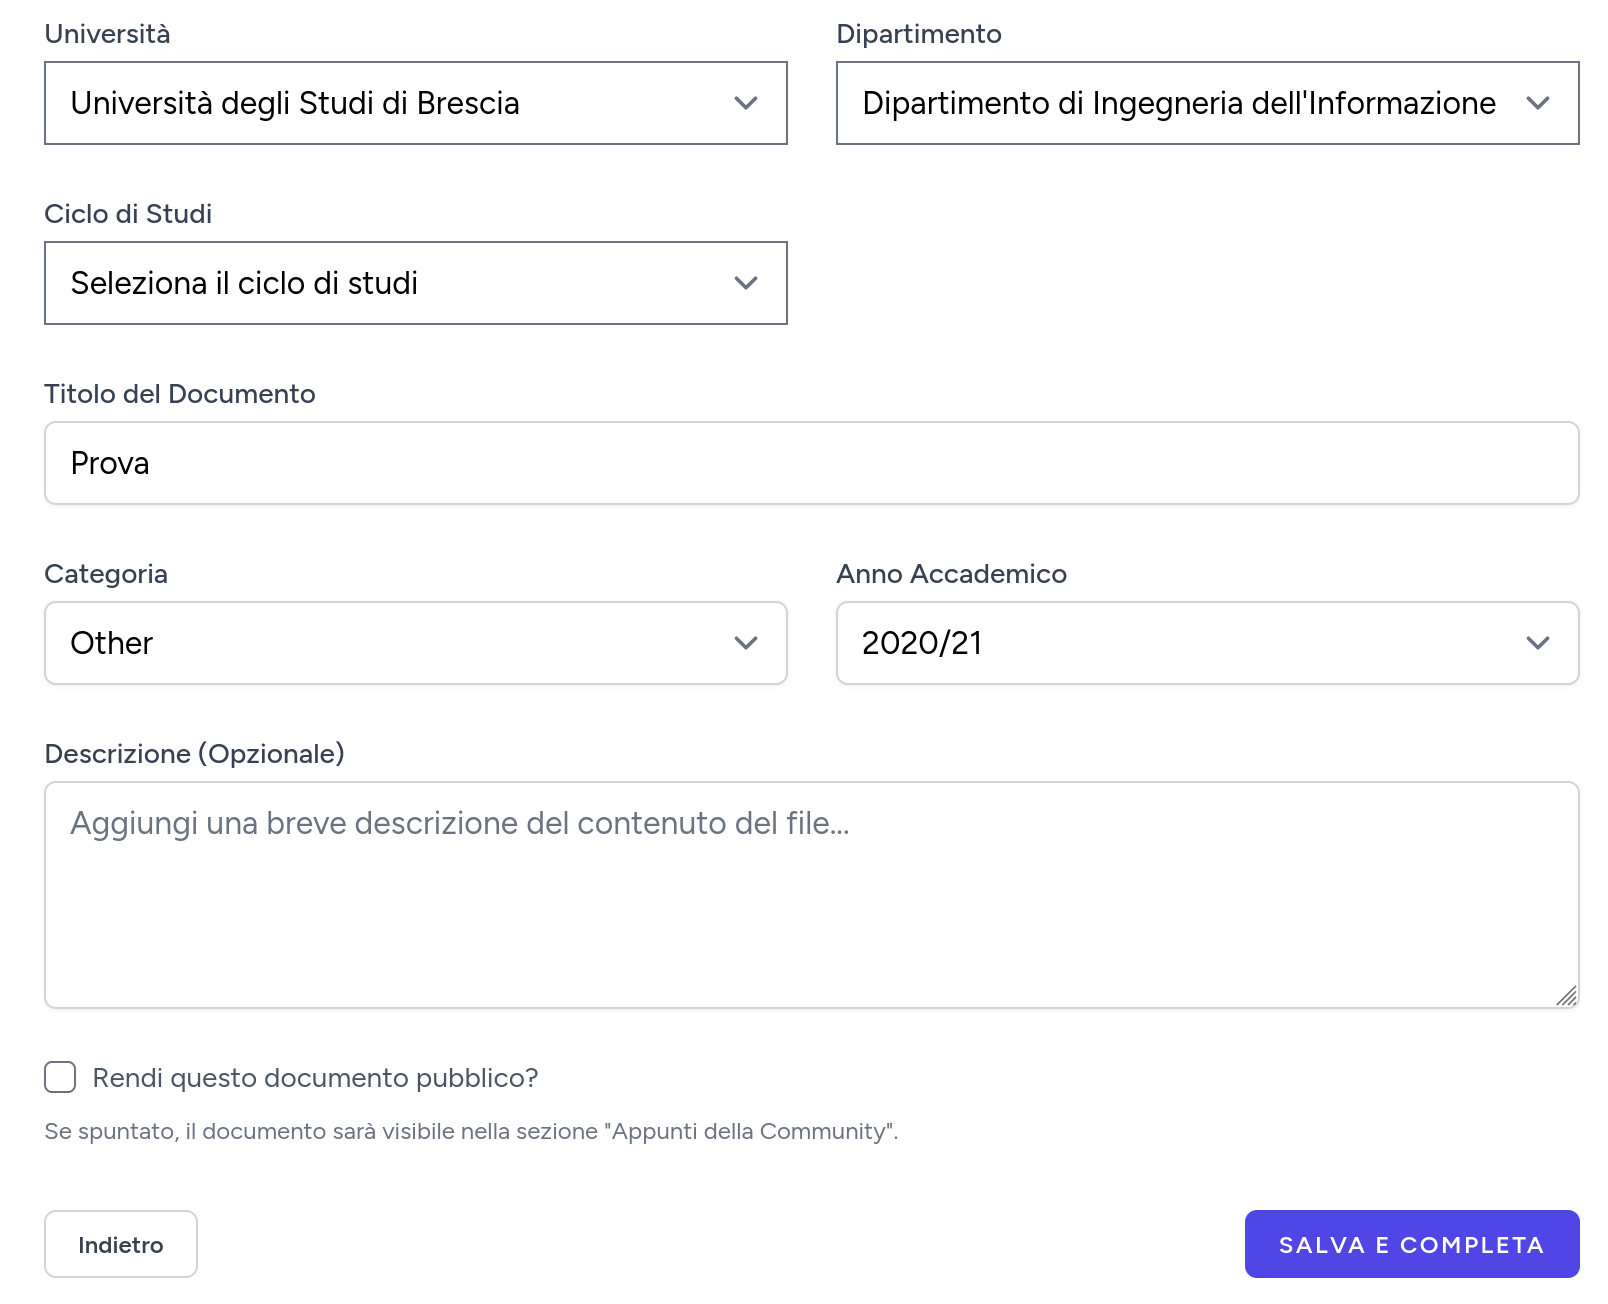
\includegraphics[width=6.5cm]{Screenshots/foglio4/Problema116.png}\hspace*{\fill}
    \vspace{10pt}
    \\
    \hline
    \textbf{Nome del valutatore} & Rinaldi \\
    \hline
  \end{tabular}
\end{table}

\FloatBarrier